%% Author_tex.tex
%% V1.0
%% developed by Techset
%%
%% This file describes the coding for SIP.cls

\documentclass{sip}%%%%where SIP is the template name

%The authors can define any packages after the \documentclass{SIP} command.

%\usepackage{amsmath} for dealing with mathematics,
%\usepackage{amsthm} for dealing with theorem environments,
%\usepackage{cite} for dealing with citations
%\usepackage{hyperref} for linking the cross references
%\usepackage{graphics} for dealing with figures.
%\usepackage{algorithmic} for describing algorithms
%\usepackage{subfig} for getting the subfigures e.g., "Figure 1a and 1b" etc.
%\usepackage{url} It provides better support for handling and breaking URLs.

\usepackage{epstopdf, epsfig}
\usepackage{caption}
\usepackage{times}
\usepackage{epsfig}
\usepackage{graphicx}
\usepackage{amsmath}
\usepackage{amssymb}
\usepackage{caption}
\usepackage{subfigure}
\usepackage{url}
\usepackage{stfloats}
\usepackage{float}


% \usepackage[pagebackref=true,breaklinks=true,letterpaper=true,colorlinks,bookmarks=false]{hyperref}

\usepackage{booktabs}

\newtheorem{theorem}{Theorem}
\newtheorem{condition}{Condition}


%The author can find the documentation of the above style file and any additional
%supporting files if required from "http://www.ctan.org"

% *** Do not adjust lengths that control margins, column widths, etc. ***
% \setlength{\textfloatsep}{5pt}

\begin{document}

\title[Semantic Segmentation of Sparse LiDAR Data]{Semantic Segmentation of Sparse LiDAR Data}

\author[
% First A. Author, \textit{et al}.
]{Jian Wu$^{1,}$$^{2}$, Xuejin Chen$^{1}$ and Qingxiong Yang$^{2}$}

\address{\add{1}{University of Science and Technology of China, Hefei, China}
\add{2}{MoonX.AI, Shenzhen, China}}

\corres{\name{Xuejin Chen}
\email{xjchen99@ustc.edu.cn}}

\begin{abstract}
In this work, we study the semantic segmentation of 3D LiDAR data in urban scenes for autonomous driving.
We proposed a method which could utilize the surface information of the ground plane.
Semantic understanding of the scene in 3D dimension is important for autonomous driving. However, the most commonly used 3D LiDAR data for autonomous driving is quite sparse. While recent work on dense point clouds segmentation has achieved promising results, points are easier to be misclassified due to the high-sparsity. In this paper, we make attempt to deal with the quite sparse 32-channel LiDAR point clouds in semantic segmentation with deep neural networks.
In particular, we incorporate the ground information with an automatic manner without any human-involved. Qualitative and quantitative experiments show that the method could
enhance the effectiveness and scene adaptability, resulting in 5\% improvement compared with existing methods.
\end{abstract}

% \keywords{Authors should not add keywords, as these will be chosen during the submission process (please refer to Section II (F) below for further details).}

\maketitle

\section{Introduction}
Scene understanding is crucial for the safe navigation of autonomous driving in complex environments.
Autonomous driving vehicles are always
equipped with both optical cameras and 3D sensors, mostly LiDAR (Light Detection And Ranging) which has wider field of view and provide significantly reliable distance
measurement robust to environmental illumination.
Based on the combined sensors, especially the LiDAR scanner which can directly get the environment information, complete environment information is created for application in computer vision.
% It is essential to not only distinguish between
% obstacles and free-space, but to also obtain a high-level task in a dynamic environment.

Semantic segmentation is the key task of autonomous driving, it
assigns a class label to each point in the input point cloud obtained by a LiDAR.
%
3D point cloud semantic segmentation has been studied for the past decade~\cite{tchapmi2017segcloud,boulch2017unstructured,riegler2017octnet,qi2017pointnet,qi2017pointnet++,landrieu2018large,jiang2018pointsift,li2018pointcnn}. 
Traditional methods use pipelines including segmenting ground from foreground objects, clustering the objects points together and performing classification based on hand-crafted features. 
Such methods are prone to low performance due to accumulation of error across successive tasks. 
With great progress in deep learning, previous methods have achieved promising results in 2D semantic segmentation~\cite{long2015fully,chen2018deeplab,kirillov2018panoptic,chen2014semantic}. 
However, there is little progress on semantic segmentation of sparse LiDAR point cloud. 
In conclusion, it can be hindered by two factors. 
Firstly, the lack of publicly available
large-scale datasets for the task of semantic segmentation in autonomous driving hinders the research. 
Secondly, unlike images, LiDAR point clouds are relatively sparse and contain a vast number of irregular, i.e. unstructured, points. 
In addition, the density of points varies
drastically due to non-uniform sampling of the environment. It can also be seen that there is a clear difference between ground and objects above the ground.
The distribution of ground points is anisotropic, but points in the obstacle area are linearly distributed.
This heterogeneous anisotropic distribution makes it significantly difficult to apply existing methods that are designed for isotropic point clouds.
%Existing methods achieve great performance when applying to the isotropic point cloud, it will be difficult to apply architecture on non-isotropic data (i.e., LiDAR point cloud).
% In Figure, we show the sparse data we used in a typical dynamic scene.

To exploit effective strategy for the challenge, in this paper we propose an approach using 3D LiDAR data from complex urban scenes by integrating ground information and deep learning methods. 
We firstly propose a strategy to automatically separate ground points and objects, which supports the subsequent feature extraction for different parts. 
In the sparse scene, objects near each other tend to be classified into the same category due to the sparsity, then we need more global information in the structure, in sparse LiDAR data, the ground makes up the large proportion of whole scene. 
We assume that it will be benefit for the task of semantic segmentation for its global structure if the ground information can be utilized completely.
Considering the compression or unfolding of landscapes in urban scenes, we use a multi-section plane extraction method to represent the ground plane in a sparse LiDAR point clouds.
%
Although only a rough segmentation for ground points is obtained at the beginning, the extracted ground points provide valuable context to eliminate the ambiguity in categorizing points of the object on the ground. 
To tackle the problem of the lack of LiDAR point cloud data, we have released the first large-scale dataset for real scene autonomous driving with full semantic segmentation of LiDAR scans. 
From the Table~\ref{dataset} we can see that unlike other datasets have many limitations for application in real scene, for example, KITTI dataset only provides bounding box for task of detection but is lack of semantic annotation. 
Without the data starvation barrier, this paper investigates which of the current state-of-the-art algorithms can be exploited and adapted for point cloud in the autonomous driving context.
After a rough segmentation of ground points, we further leverage effective deep learning method to extract more reliable features for the ground and objects.   

Qualitative and quantitative experiments show that the combination of a large amount of constraint data significantly improves the effectiveness and scene adaptability of the classifier.

The remainder of this paper is organized as follows. Related work is discussed in Sect. II. In Sect. III, the proposed method is presented.
Then, we present the experimental results in Sect. IV and draw conclusions in Sect. V.





\begin{table*}[!t]
\setlength{\abovecaptionskip}{0cm}
\setlength{\belowcaptionskip}{-20cm}
\captionsetup{font={large}}
\caption{Compared with different 3D point cloud dataset for semantic segmentation. }
\label{dataset}
\begin{center}
% \small
\setlength{\tabcolsep}{0.8pt}
{\begin{tabular}{lccccccccc}
% \toprule
\hline
 & S3DIS~\cite{armeni20163d} & Semantic3D~\cite{hackel2017semantic3d} & ScanNet~\cite{dai2017scannet} & KITTI~\cite{geiger2012we} &Oakland3D~\cite{Munoz-2009-10227} & Apolloscape~\cite{huang2018apolloscape} & DF-3D~\cite{timmurphy.org}& Ours\\
\hline
Scene & Indoor & Outdoor & Indoor & Outdoor & Outdoor& Outdoor  & Outdoor&Outdoor\\
Sparse/Dense & Dense & Very Dense & Dense & Sparse & Dense & Dense  & Sparse &Sparse  \\
Ground Annot. & Y & Y & Y & N & N & N & N & N  \\
LiDAR & - & - & - & 64E & - & -  & 32E &32E\\
\hline
\end{tabular}}{}
\end{center}
\end{table*}

\begin{figure*}[hpt]
    \centering
    % \includegraphics[width=0.88\textwidth]{result1.png}
    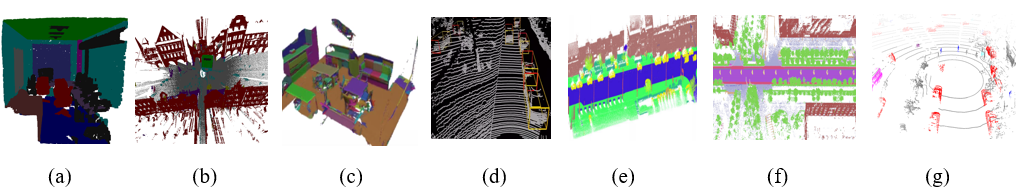
\includegraphics[width=0.92\textwidth]{diffdata.png}
    \captionsetup{font={small}}
    \caption{Different 3D point cloud dataset for semantic segmentation. (a) S3DIS. (b) Semantic3D. (c) ScanNet. (d) KITTI. (e) Oakland3D. (f) Apolloscape. (g) DF-3D.}
    \label{fig:diffdata}
\end{figure*}




\section{Related Work}

\paragraph{Scene Understanding in Autonomous Driving.}
Autonomous driving has received widespread attention and development in recent years.
Scene understanding is one of the key building blocks of autonomous driving in dynamic, real-world environments.
Scene understanding tasks are mainly divided into object detection and semantic segmentation.
Earlier works~\cite{maturana2015voxnet,qi2016volumetric,song2016deep,wang2019frustum,shi2018pointrcnn} have made great progress in the detection task of autonomous driving.
However, the bounding box representation can only provide rough localization information, but lacks sufficient semantic details. 
Semantic segmentation provides more detailed point-wise segmentation, which is vital for visual perception tasks of autonomous driving. Such semantic segmentation not only provides important information for vehicle decision-making, but also provides a powerful auxiliary role for precise positioning, which is essential in many autonomous driving applications.
Previous approaches have achieved promising results in 2D semantic segmentation~\cite{yang2018segstereo,wang2018understanding,teichmann2018multinet} for autonomous driving.
These techniques well exploit the texture information in 2D images, but they can not be applied to 3D point clouds that are irregular, i.e. unstructured in 3D domain.





\paragraph{Semantic Segmentation of Point Clouds.}
Relative to image segmentation, there is very little literature on point cloud semantic segmentation.
Traditional approaches~\cite{chen2003visual,sun2009concise} for point cloud semantic segmentation are done utilizing complex pipelines, composed of many successive steps such as: ground removal, point cloud clustering, feature extraction as presented in~\cite{feng2014fast,himmelsbach2008lidar}. 
However, these methods usually require a lot of parameters and are difficult to tune.
Deep learning has been widely used in 3D point cloud segmentation, and great progress has been made by learning more comprehensive and discriminative features in recent years. 
~\cite{qi2016volumetric,tchapmi2017segcloud,wu20153d} propose to represent the
point cloud as a high-dimension volumetric form which can be applying with 3D convolutional neural networks. This representation is constrained by its resolution due to data sparsity and redundant computation of
3D convolution which is not suitable for LiDAR point clouds.
PointNet~\cite{qi2017pointnet} learns point-wise features with multilayer perceptrons (MLPs), and extracts global features with max-pooling. 
It is the first attempt for using as inputs the raw, un-orderered point clouds and apply symmetrical operators that are able to deal with ordering problem of 3D point cloud.
For this purpose, max pooling is used to extract global and permutation-invariant features.
However, it loses the ability to capture local structures, which limits its generalizability to complex scenes.
The limitations were later tackles by designing a hierarchical structure to capture local region features in PointNet++~\cite{qi2017pointnet++}. 
By exploiting individual PointNet architectures in a local area, it captures local information and then applies this hierarchical architecture to exploit increasing contextual scales in metric spaces.
%
Although good results have been achieved in indoor scenes, based on our experiments, neither method can be well generalized to large-scale point clouds in autonomous driving scene.
PointCNN~\cite{li2018pointcnn} is proposed to learn a transformation of the input points for the feature weighting and point reordering and then apply typical CNN architecture to process irregular and unordered 3D points.
Inspired by the SIFT feature extractor~\cite{lowe2004distinctive}, PointSIFT~\cite{jiang2018pointsift} employs local octant directional vectors as feature extraction layers which showing great results in indoor scene segmentation.
Other methods, such as OctNet~\cite{riegler2017octnet} uses octree to represent features of point clouds.
Unfortunately, the method also requires drastically increasing memory and is not suitable for large-scale LiDAR point clouds.


\paragraph{Semantic Segmentation of Large-Scale LiDAR Point Clouds.}
The main challenge of LiDAR perception in general is the sparse and large-scale nature of point cloud data.
To deal with large-scale outdoor point clouds, SPG~\cite{landrieu2018large} manages to summarize the local
relationships in a similar fashion to PointNets by coarsely segmenting a point cloud into a superpoint graph. Superpoints are locally coherent, geometrically homogeneous groups of points that get embedded by feature extractors. 
Promising improvement has been made by SPG compared to previous methods on dense point cloud data.
However, for sparse LiDAR point clouds, due to the heavy workload for data annotating, large-scale LiDAR data for supervised 3D semantic segmentation is very scarce which will hinder the development of semantic segmentation in autonomous driving.
Some approaches was proposed for the semantic segmentation of LiDAR point clouds represented as 2D image views~\cite{wu2018squeezeseg,wang2018pointseg} or using synthetic data~\cite{chen2017multi,varga2017super}.
%
SqueezeSeg~\cite{wu2018squeezeseg} use a spherical projection of the point cloud enabling the usage of 2D
convolutions and CRF for semantic segmentation. 
This representation allows to perform the segmentation via utilizing a light-weight fully convolutional network for semantic segmentation, the last step is to obtain the unprojected results in 3D world from 2D segmentation results in image view.
%
Following that, PointSeg~\cite{wang2018pointseg} improves the CRF process of SqueezeSeg to give more consideration to local information.
SqueezeSegv2~\cite{wu2018squeezesegv2} improves the model of SqueezeSeg with a Context Aggregation Module and by considering focal loss and batch normalization to improve its robustness and quality of segmentation.
%
However, their results often lack of accuracy which limits their usage in real scenarios, especially on small objects classes such as cyclists or pedestrians.
There also exists a large gap between real sparse 3D point clouds and 2D representation or synthetic data.




\begin{figure}[t]
\setlength{\abovecaptionskip}{30pt}%
\setlength{\belowcaptionskip}{1pt}%
    \centering
    % \setcounter{MYtempcnt}{\value{figure}}
    % \setcounter{figure}{2}
    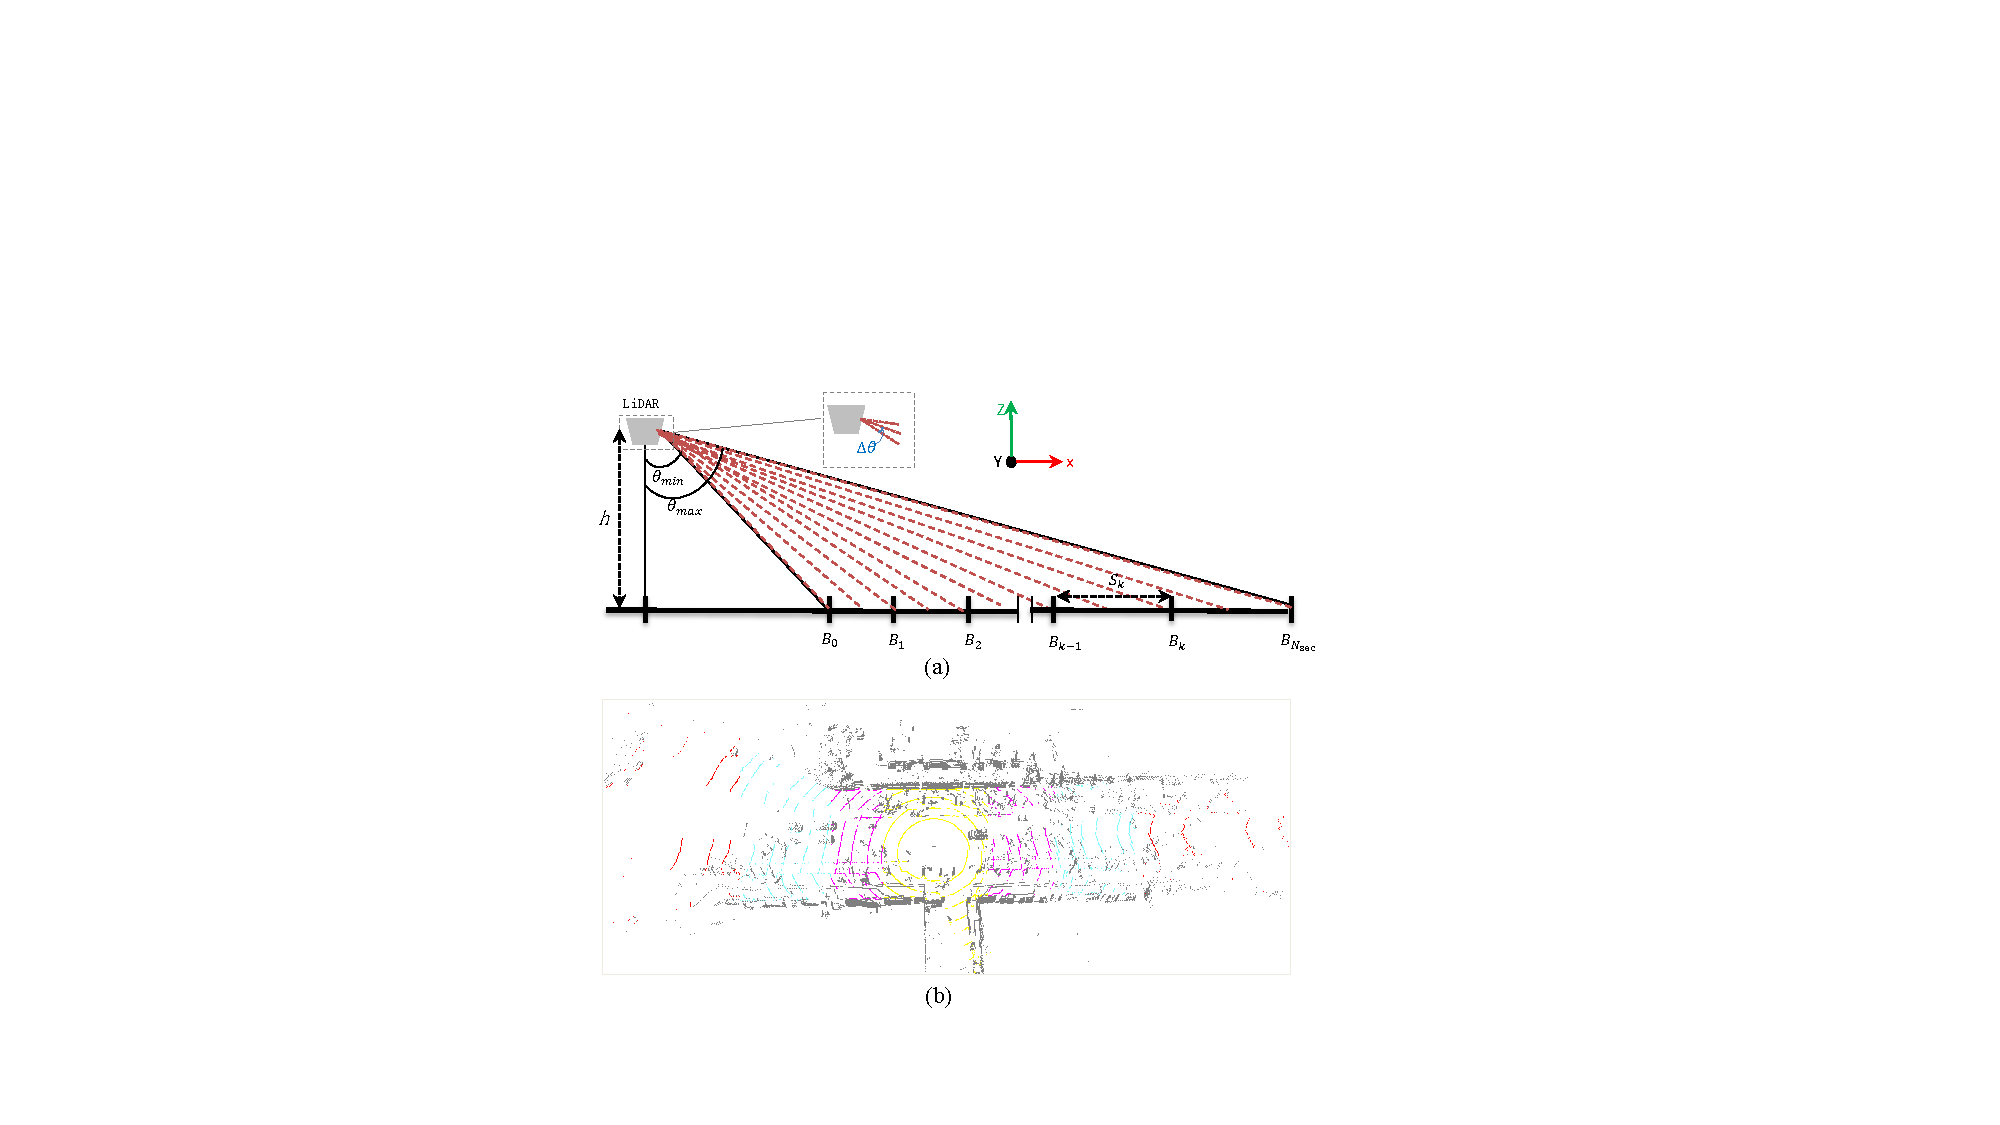
\includegraphics[width=\columnwidth]{lidar.pdf}
    % \includegraphics[width=0.9\textwidth]{result2.png}
    % \setcounter{figure}{\value{MYtempcnt}}
     \captionsetup{font={small}}
    \caption{Multi-section ground plane segmentation. (a) Divided by scanning lines. Each red dashed line represents a Velodyne-32 LiDAR scan ray. (b) Extracted ground points in multiple sections. Different colors illustrate different sections.}
    \label{fig:lidarscan}
\end{figure}

\begin{figure*}[ht]
	\begin{center}
		% \fbox{\rule{0pt}{2in} \rule{0.9\linewidth}{0pt}}
		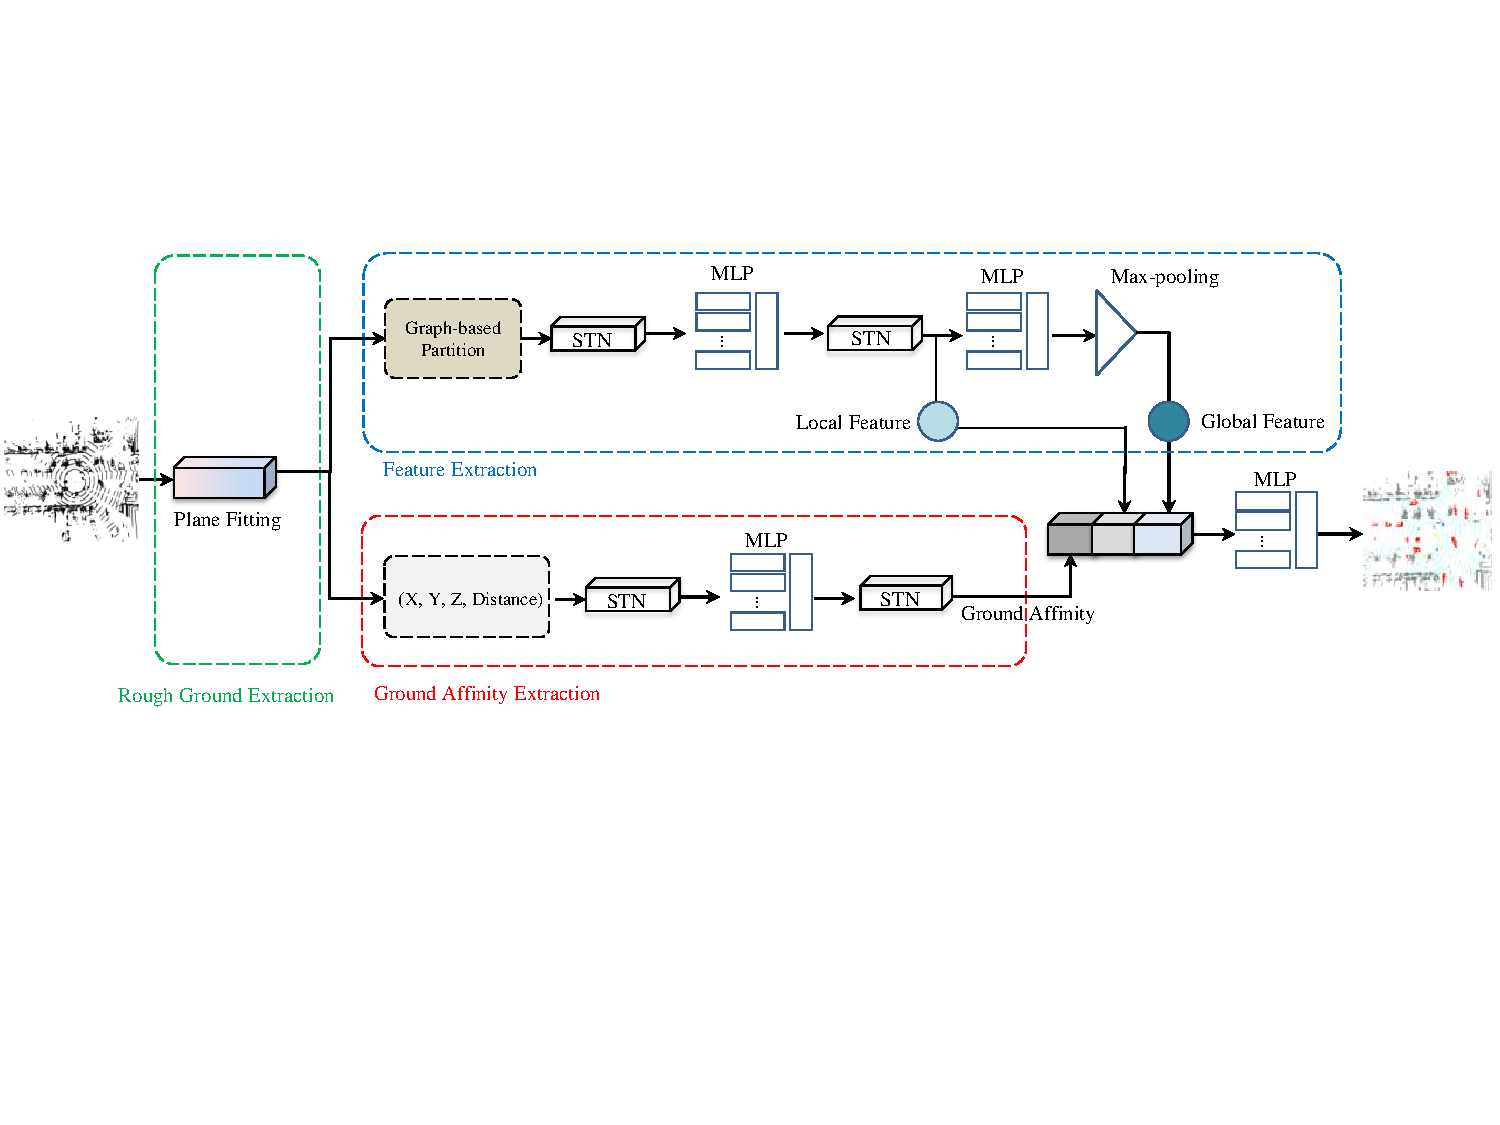
\includegraphics[width=1.0\linewidth]{framework.pdf} 
	\end{center}
	\caption{The proposed framework for point cloud semantic segmentation. We first roughly extract ground points by multi-section plane-fitting from the input point cloud. Then the point cloud is partitioned into multiple parts for feature extraction. For each part, local features and global features are extracted by utilizing MLPs. The roughly segmented ground and object points are fed into our distance feature extraction module to capture relationship between object points and ground points. By concatenating the ground affinity feature, local feature, and global feature, each point is classified into $K$ categories for the final prediction of semantic labels. }
	% \label{fig:long}
	\label{fig:semi-global}
\end{figure*}
\section{Methods}
As shown in Figure \ref{fig:semi-global}, our framework of 3D point cloud semantic segmentation mainly consists of three parts, including a rough ground extraction module which roughly segments the input point
cloud into ground points and object points, a feature extraction module to extract local and global features, a ground affinity extraction module to build the relationship between the ground points and object points.
In the following paragraphs, we will describe each of the above
modules in terms of the functionality and the specific architectures.

\subsection{Rough Ground Extraction }\label{sec:ground}
For the point distribution of ground and objects above the ground are various which makes it significantly difficult to apply existing methods that are designed for isotropic point clouds, we first perform a rough segmentation of the input LiDAR point cloud. 
We define the input LiDAR point cloud as $\mathcal{P}=\{p_1,\ldots, p_N\}$, which will be divided into two subsets $\mathcal{P}_{ground}$ and $\mathcal{P}_{objects}$ via fitting the ground planes. 
The autonomous driving scene is extremely complex, the ground is usually not a perfectly regular plane, meanwhile, the LiDAR scanner measurements will introduce signal noise when the scanning distance is long. 
From this perspective, a single plane model can not represent the real ground surface in practice. 
Multi-section plane fitting method is used in our pipeline to fit the ground and extract ground points from the input LiDAR point cloud. 
Our approach is based on the assumptions that most objects like vehicles and pedestrian locate on the ground in autonomous driving scene, to this end, we suppose that when the ground can be well segmented the accuracy of other categories can be improved as well. 
Meanwhile, we empirically find that the ground plays an important role in sparse point clouds segmentation, the objects were consisted with the number of points, mutual interference among the points will cause the error predicted of the objects.

Firstly, the input point cloud is divided into a plurality of regions along the driving direction of the vehicle.
%
In general, the scanning lights are uniformly distributed at intervals of angle $\triangle\theta$, so the point density varies at different distances of scanning.
We divide the input point cloud based on the same angular intervals, as illustrated in Figure~\ref{fig:lidarscan}(a).
%
Taking the point cloud in front of the LiDAR equipment as an example, we divide these points into $N_{sec}$ parts by calculating a set of area boundaries $\{B_k\}_{k=0,\dots,N_{sec}}$ along the driving direction as
%Instead of dividing the scene with equal size,
%
\begin{equation}\label{111}
B_k=h\tan(\theta_{min}+k\mu\triangle\theta),\; k=0,...,N_{sec} ,
\end{equation}
where $h$ is the height of the LiDAR equipment on the ground plane.
% which is an intrinsic parameter from the device.
$\theta_{min}$ and $\theta_{max}$ represent the range of the scanning angles of the LiDAR equipment.
$N_{sec}$ is the default number of sections, and $\mu$ denotes the number of scanning rays in each section.
All the 3D points whose $x$ coordinates fall into $(B_{k-1}, B_k\rbrack$ are splited into
the section $S_k$.
For each divided section along the driving direction of vehicles, we use RANSAC~\cite{fischler1981random} to estimate a ground plane. 
Since there are many points of both the ground and objects, we first need to select the possible ground points whose $y \in [y_{l}, y_r]$ and $z\in[z_u, z_b]$ to reduce noise in the step of fitting plane.
Then a plane $P_k$ is fitted for these selected points using RANSAC.
%
After the ground part of the entire point cloud is extracted, the obtained ground plane is used to distinguish non-ground points from ground points by distance measurement.
For a point at position $\mathbf{p}=(x,y,z)$ in a section $S_k$, if its distance to the plane $d(p,P_k)>\sigma$, it is temporally divided as an object point. Otherwise, it is divided as a ground point.
Figure~\ref{fig:lidarscan}(b) shows an example of extracted ground points in multiple sections in a sparse point cloud.


\subsection{Feature and Affinity Extraction}
Extracting and representing features from extremely sparse and large-scale point cloud data is a challenging task. 
Previous works usually attempt to utilize the 2D image representation by projecting from the 3D LiDAR data, however, their results often lack of accuracy for the limitation of resolution of 2D view image, therefore it has many hinders in real scenarios, especially on small objects classes such as cyclists or pedestrians.
Recent researches such as~\cite{landrieu2018large} have shown the successful application of graph-based representation of LiDAR point clouds in large-scale urban scenes.
The novel method does not classify individual points, but divides them into simple geometric superpoint structures to reduce the scale of the entire point cloud. Then a graph structure is constructed to capture the relationship between adjacent superpoints.
In our architecture, we also apply a graph-based partition step of the input LiDAR point cloud.
%
%
Since the input large-scale point cloud $\mathcal{P}$ has been divided into ground points $\mathcal{P}_{ground}$ and objects $\mathcal{P}_{objects}$ in the previous chapter, in our architecture we run graph-based partition on the ground points and object points separately.



After graph-based partition step, we choose the PointNet~\cite{qi2017pointnet} as feature extraction architecture for its simplicity and efficiency, it is applied for each set of points clustered to the same superpoint. 
In order to learn spatial information of different parts of point clouds, each superpoint graph is rescaled to the unit sphere before extracting steps.
Figure \ref{fig:semi-global} illustrates the detail architecture in the feature extraction module.
We employ a spatial transform network (STN) which combined with T-Net and transform matrix to align the points in each superpoint to a canonical space in the feature level.
After the second STN, we obtain a $64$-D feature vector for each point as its local feature and $512$-D global feature vector for the superpoint after two MLPs and a max-pooling layer.
%
For each point in the point cloud, we concatenate its local feature and global feature and get a $576$-D feature vector.

In our architecture, we also build the relationship between the ground points and the object points above the ground by utilizing the distance to the ground surface as an extra channel for feature embedding. Specifically, as ground affinity extraction module in Figure \ref{fig:semi-global} shows, we take the position and distance as input which is represented as $(x,y,z,d)$, where $d$ represents the distance of the point against to the fitted ground plane, allowing us to associate a height with respect to the ground plane. 
Then the (${x, y, z}$) coordinates and distances are separately processed by partial PointNet with STNs and MLPs. 
After the embedding module, we acquire the features embedded with ground affinity in the dimension of $N\times512$ which carry more information of LiDAR point cloud. 
We concatenate the ground affinity feature with the local and global features which are obtained in the step of feature extraction with $N \times 576$. 
Finally, a few MLPs are used to output per-point scores for the $K$ categories, then we will obtain the final results of semantic segmentation.

\subsection{Weighted Loss Function}\label{sec:loss}
Our entire framework is supervised in a weakly supervised manner, in which ground information is obtained automatically, as described in Sec.~\ref{sec:ground}.
%
Although not exactly the \emph{real} ground-truth, we produce pesudo labels to provide weak supervision for the network training without any human-involved efforts.
%
We empirically found that there is a severe imbalance in the number of categories in the LiDAR point cloud dataset, which are biased towards dominant classes rather
than others from the perspective of having higher number of instances. 
For instance, number of instances for \emph{vehicles} class is greater than others like \emph{pedestrians} and \emph{bicycles}, meanwhile the background points occupy most of the scenes.
The imbalance condition may easier lead to either miss or wrongly classifying whole classes points.
%

In order to solve the imbalanced point cloud datasets problems and increase the accuracy of small objects, we utilize a class-balanced cross-entropy loss,
which can not only classify different objects correctly, but also enhance mean IoU measurement metric of point-wise classification, 
given as
%
\begin{equation}\label{eq:cbloss}
L_{weighted}=-\frac1N_t\sum_{i=1}^{N_t}\sum_{k=1}^{K}\alpha_k \vb{y}_{ik}\log \vb{p}_{ik} ,
\end{equation}
where $\vb{p}_{ik}$ represents the probability of the $i$th point belonging to the $k$th category, with a total of $N_t$ points in the entire training part.
We compute the weight for each category as $\alpha_k=f_{med}/f_k$, where $f_k=\sum^M_{i=1} N_{ik}$ is counting for the total number of points of the $k$th category in the whole training set.
$f_{med}$ is the median of $f_k$ over all the $K$ categories.  









\begin{figure*}[hpt]
\setlength{\abovecaptionskip}{-10pt}
\setlength{\belowcaptionskip}{-0.cm}
    \centering
    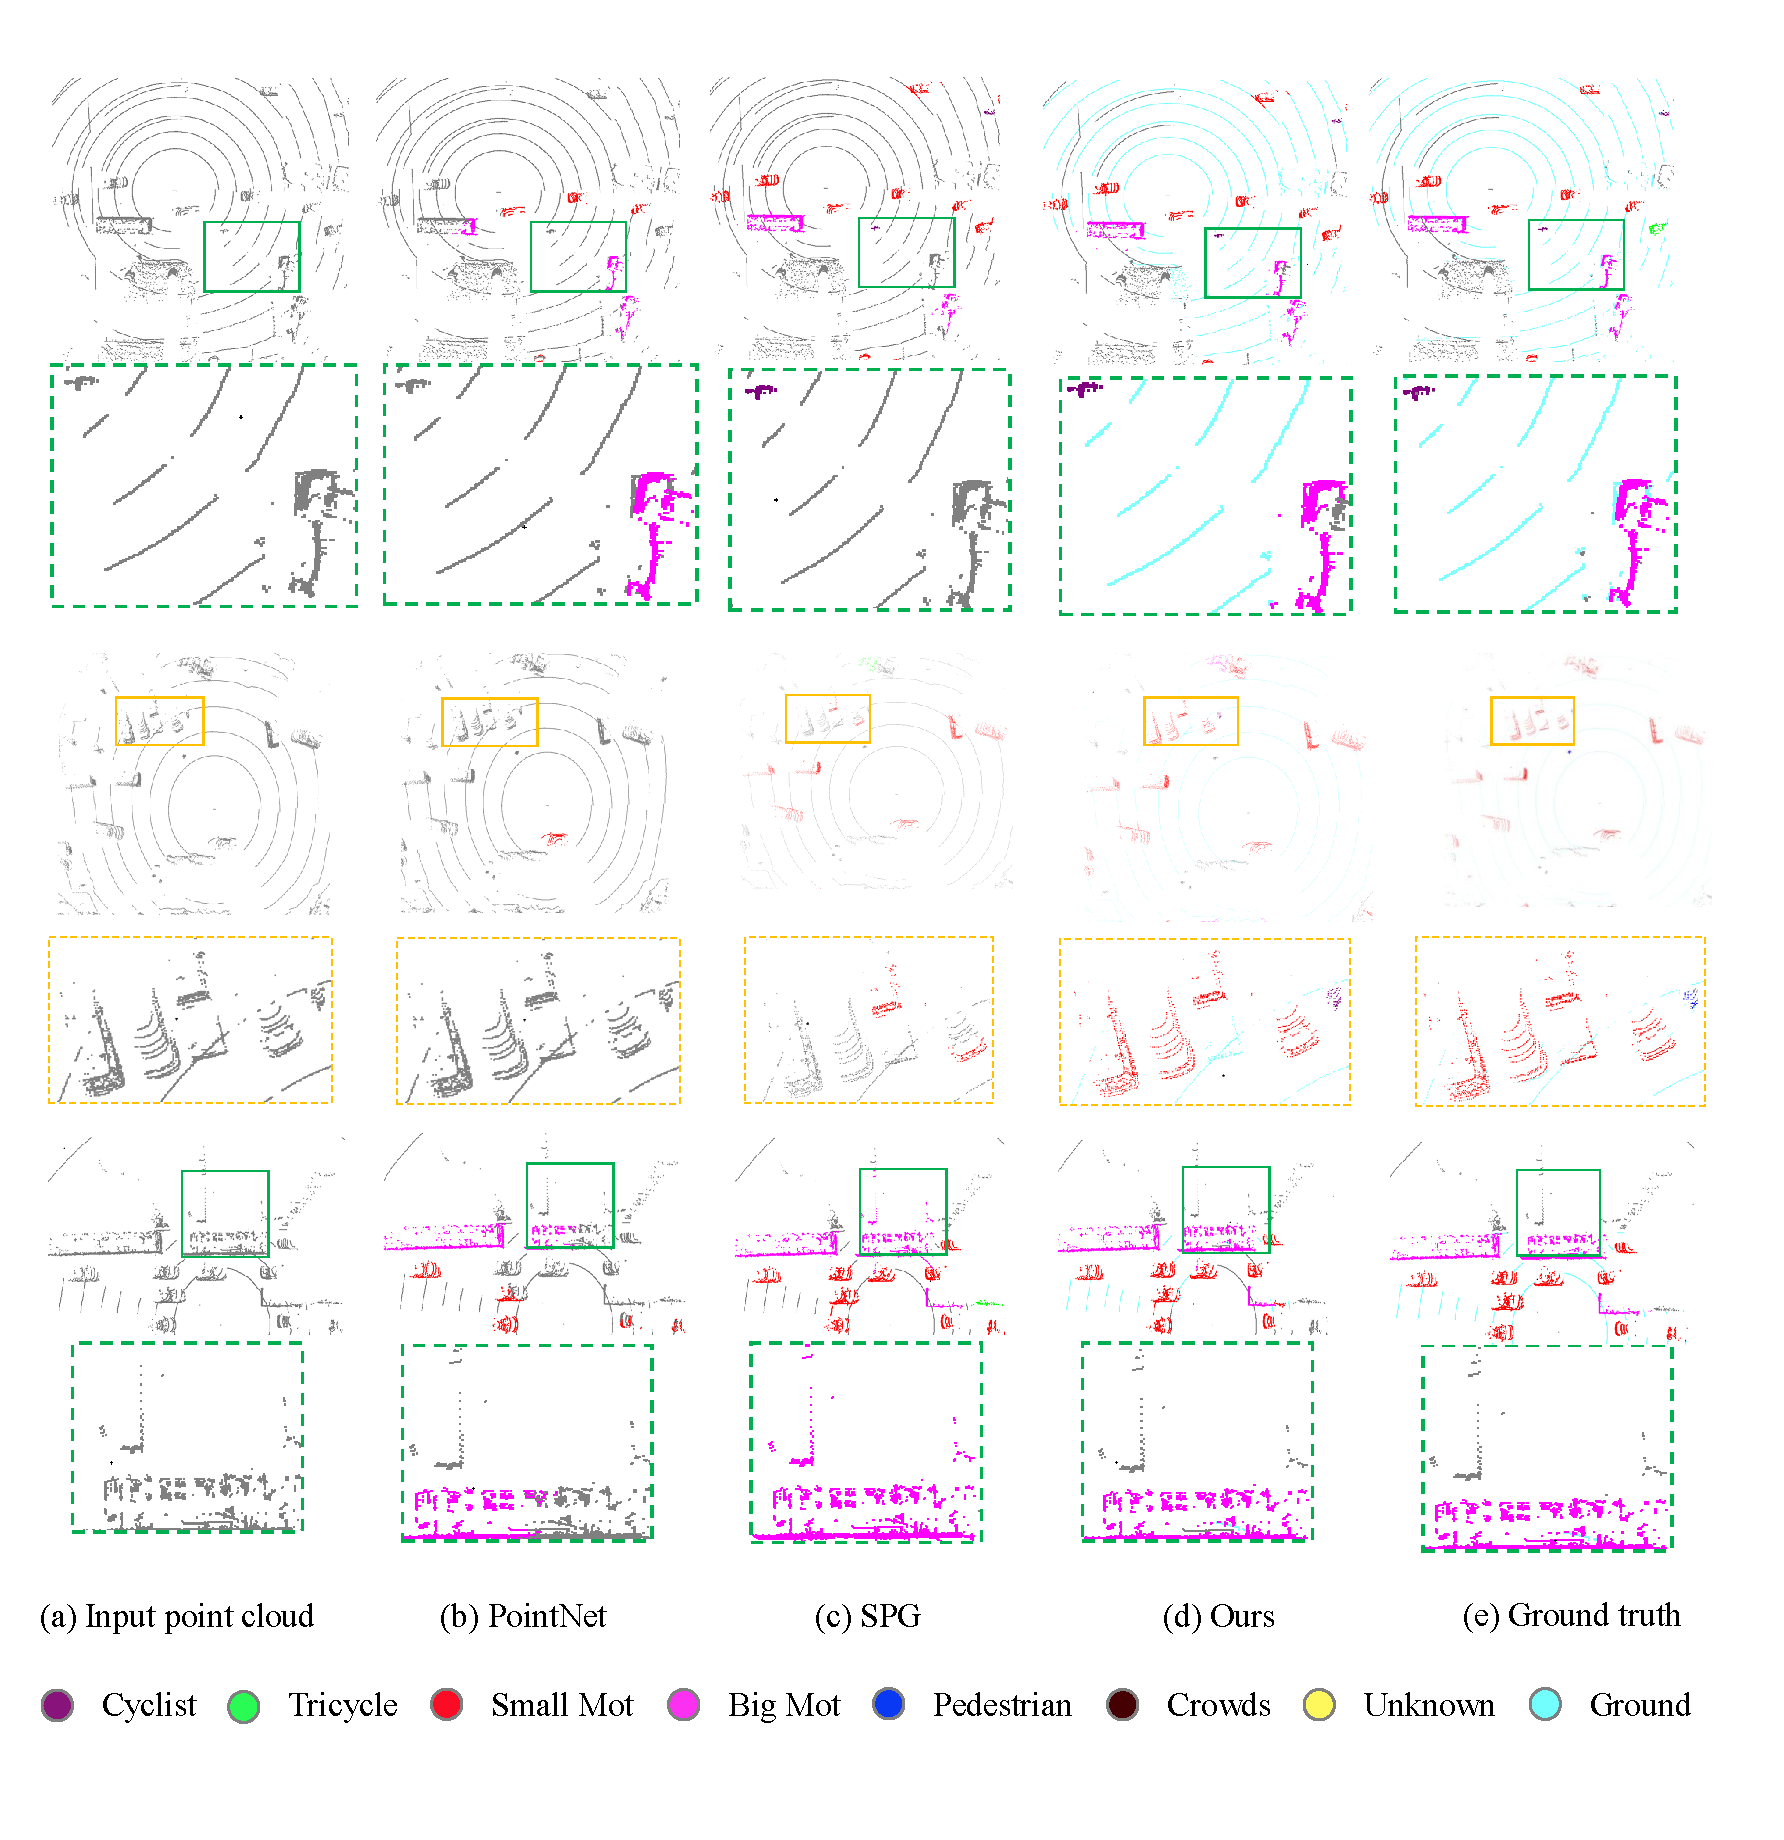
\includegraphics[width=0.91\textwidth]{result.pdf}
    \captionsetup{font={small}}
    \caption{Visual performance on point clouds semantic segmentation.}
    \label{fig:vis}
\end{figure*}


\section{Experiments}\label{sec:exp}
In this section, we evaluate our framework on two datasets of sparse LiDAR point clouds, the DF-3D semantic dataset~\cite{timmurphy.org} and a newly collected dataset in urban road scenes with our own Velodyne HDL-32E LiDAR device which is equipped on an autonomous driving car.
A series of quantitative and quantitative comparisons will be shown to prove the superiority of our ground-aware approach.

\subsection{Datasets}
The LiDAR devices that continuously launch and receive multi-beams lasers at 360 degrees, they are now key components of perception systems as they provide an accurate 3D representation of the autonomous driving scene.
Recent years more and more companies (e.g., Uber, Baidu, Alibaba etc.) adopt 32-channel LiDAR device equipped on autonomous cars in real applications.
The 32-channel LiDAR device is much cheaper compared to the 64-channel LiDAR device, generally less than half price.
Meanwhile, the 32-channel LiDAR device has a smaller size which can be more easier to equip on the automatic car, making it more efficient for application in real complex scene.
While the 64-channel LiDAR point cloud data has also been used in previous researches, for instance, the KITTI dataset~\cite{geiger2012we} is applied for the task of 3D object detection in autonomous driving. 
However, for the task of 3D point cloud semantic segmentation, the more challenging and much sparser point clouds captured by 32-channel LiDAR device has not been well studied yet.
This paper focuses on the semantic segmentation of 3D LiDAR point clouds captured by 32-channel LiDAR device.
\begin{figure}[H]
    \centering
    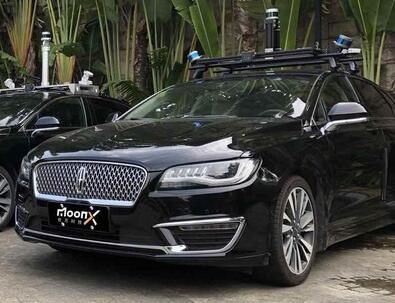
\includegraphics[width=0.9\columnwidth]{car1.jpg}
    \caption{Our autonomous car for the scanning dataset in various environments. It is equipped with some cameras, LiDAR sensors for perception. }
    \label{fig:teas}
\end{figure}


\paragraph{DF-3D Dataset.}
The DF-3D dataset~\cite{timmurphy.org} is collected by Alibaba$\textsuperscript{\textregistered}$ for 3D point cloud semantic segmentation of autonomous driving scene.
It was collected with a Velodyne HDL-32E LiDAR sensor (a famous and widely-used LiDAR device) on a moving vehicle on complex environment, not only inner city traffic, residential areas, but also highway scenes and countryside
roads.
%
This dataset contains 80,000 point-wise labeled 3D scans, which provides 50,000 for training and 30,000 for testing.
Each 3D scan contains about 50,000 3D points.
The annotations contain seven classes (\emph{cyclist, pedestrian, tricycle, small mot, big mot, crowds, and others}) in total.
A point of the "others" category is belong to non-moving or moving objects on effective driving area of streets, but does not belong to any of the other six classes.
The background and ground points are not labeled in this dataset. 
We treat these points as the "unlabeled" category in our segmentation network.
For the ground truths for the test set are not available, we randomly split the training part into a new training set and a new testing set, which containing 35,000 and 15,000 frames, respectively.
Each 3D point is contained with its position $({x, y, z})$ in the global coordinate system.




\paragraph{Semantic-LiDAR Dataset.}
In addition to the DF-3D dataset, in order to perform a thourough evaluation, we collected a new dataset by using the Velodyne HDL-32E as our environment perception device. 
This sensor scans the surrounding area by 32 rotating laser beams, and each scan line has 2160 laser points at different horizontal angles, each data frame is associated with a time log for synchronization. 
The GPS/IMU data are logged at 100 Hz, the LiDAR data are recorded at 10 Hz.
The point cloud data is captured with the device same as the DF-3D dataset, with a minor difference for the annotated categories.
In contrast to the DF-3D dataset, we define five categories including \emph{cyclist, pedestrian, tricycle, car, and others}.
Our dataset contains 3,000 frames in total, we provide 2,400 frames for the training set and 600 frames as the test set.
Both of the two datasets are publicly available through a benchmark website and we provide only the training set with ground
truth labels and perform the test set evaluation online.

\paragraph{Evaluation Metrics.}
To quantitatively evaluate our method and compare to other approaches, in our experiments, we use the commonly applied metrics in prior works~\cite{hackel2017semantic3d} for large-scale outdoor scenes: the Intersection over Union(\emph{IoU}) over each class, the average IoU (mIoU) over all classes, and the overall accuracy (OA).

\begin{table*}[!t]
% \large
 \captionsetup{font={large}}
\caption{Compared with different methods on the DF-3D dataset.}
\label{diff method}
% \resizebox{10pt}{50mm}
\setlength{\tabcolsep}{6pt}
\begin{center}
{\begin{tabular}{lccccccc|cc}
\hline
 Methods& sm allmot & crowds & pedestrain & cyclist &tricycle & bigmot &others & m\emph{IoU} (\%) & \emph{OA}. (\%)  \\
\hline
3D FCN~\cite{li20173d} & 22.7 &1.2  &0.6  &4.7  &2.1 &21.4  &6.2  &8.4 &10.1 \\
PointNet~\cite{qi2017pointnet} & 45.8 &3.1  &2.2  &8.4  & 5.3&54.4  & 13.3 &19.0 &22.6 \\
PointNet++~\cite{qi2017pointnet++} &48.3  &2.7  &3.9  &10.5  &5.6 &50.1  &12.9  &19.2 &23.0 \\
PointCNN~\cite{li2018pointcnn} & 50.4 & 3.3 &6.8  &8.2  &6.2 &46.9  &15.2  &19.6 &23.3 \\
SPG~\cite{landrieu2018large} & 68.5 & 9.8 & 8.4 & 19.2 & 7.3& 60.1 & 23.2 & 26.8&30.2 \\
Ours & \textbf{70.4} & \textbf{10.3} & \textbf{10.8} & \textbf{21.9} & \textbf{10.2} & \textbf{68.1} & \textbf{23.9} & \textbf{30.8} &\textbf{33.6} \\
\hline
\end{tabular}}{}
\end{center}\vspace{-2mm}
\end{table*}

\begin{table*}[!t]
 \captionsetup{font={large}}
\caption{Performance evaluation on the Semantic-LiDAR dataset.}
\label{diff our data}
% \resizebox{10pt}{50mm}
\setlength{\tabcolsep}{7pt}
\begin{center}
{\begin{tabular}{lccccc|cc}
% \toprule
\hline
 Methods& vehicle & cyclist & pedestrain &tricycle & others & m\emph{IoU} (\%) & \emph{OA}. (\%)  \\
% \midrule
\hline
3D FCN~\cite{li20173d} &48.5  &1.3  &1.2  &1.2  &9.4 &12.3  &13.8   \\
PointNet~\cite{qi2017pointnet} & 69.5 &0.7  & 5.2& 13.8 & 2.2 &13.1 &14.8 \\
PointNet++~\cite{qi2017pointnet++} &73.2  & 2.6 &9.8  &\textbf{18.6}  &5.5 &21.9  &23.7   \\
PointCNN~\cite{li2018pointcnn} & 70.4 &8.3  &10.5  &14.2  &7.7  &22.3  &24.5 \\
SPG~\cite{landrieu2018large} & 78.5 & 3.5 & 8.5 & 16.5& 4.2 & 22.2&24.1 \\
Ours & \textbf{80.7} & \textbf{16.7} & \textbf{12.2} & 17.2 & \textbf{10.3} & \textbf{27.4} &\textbf{29.3} \\
\hline
\end{tabular}}{}
\end{center}\vspace{-2mm}
\end{table*}
\paragraph{Implementation Details.}
Our proposed architecture is implemented by utilizing PyTorch~\cite{paszke2017automatic} framework and trained on four GTX 1080 Ti GPUs.
The optimization is achieved by the Adam optimizer~\cite{kingma2014adam} with the initial learning rate as 0.01.
The batch size is set as 20 in our experiments.
The model was trained for 300 epochs with the learning rate decay of 0.7 at epochs 150, 200, and 250.

\subsection{Quantitative Evaluation}
From the Table \ref{diff method}, quantitative results are showed on the 3D-DF dataset, our approach is compared with other previous state-of-the-art methods, while the comparison on our newly collected Semantic-LiDAR dataset is shown in Table ~\ref{diff our data}.
From the results, we can see that our method enhances the evaluation metrics compared with applying other approaches for 3D point cloud semantic segmentation on both datasets.


More importantly, the detection or semantic segmentation of small objects is a challenging problem in the vision community~\cite{kampffmeyer2016semantic,lin2017feature,wang2018understanding}. 
As the results shown in Table~\ref{diff method} and Table~\ref{diff our data}, previous methods perform poorly on the small objects (e.g., \emph{crowds, pedestrian}, etc.) in such sparse datasets. 
In contrast, our method is robust for small objects. For instance, the \emph{pedestrian} category in the LiDAR data we used only has several points in the scene, but in our method, it performs significantly better than state-of-the-arts methods.


Previous methods have difficulties to accurately segment points for small objects, such as \emph{crowds, pedestrian, and tricycle} in such sparse point clouds.
For instance, the \emph{pedestrian} category in the LiDAR data only has several points in the scene.
%







\subsection{Qualitative Performance}

From the Figure~\ref{fig:vis} we can see the quantitative results in 3D-DF dataset, which contains fine-grained semantic categories (e.g., crowds and pedestrian, big mot and small mot.) that can effectively illustrate the model performance.
From the quantitative results we can see that our framework performs better than other methods in many aspects.
Especially, we show the results in details in close-up views in Figure~\ref{fig:vis}.

In the first example (the green box), our method correctly segments all the small objects and big objects above the ground, while the other methods either fail to segment cyclist or fail to classify big vehicle in this example.
Our approach is robust for those \emph{small mot} points which are far away from the LiDAR device, demonstrating the benefit from relationship which is built between objects and the ground.
In the second example, from the orange box we can see when many vehicles are crowded in a small area, previous methods can hardly segment the vehicles, or misclassify the vehicles that are close to each other.
In comparison, they are correctly classified with our novel approach.
%
In the green box of third example, we can see that our approach is robust for \emph{big mot} which is easier to be misclassified in some complex urban scenes. From the visualized results, we can get the conclusion that our approach can achieve great performance and reduce the misclassified problem in 3D point cloud semantic segmentation in autonomous driving scene.










\section{Conclusion}
In our work, we presented an effective architecture for performing semantic segmentation of large sparse LiDAR point clouds by implicitly incorporating the ground information. 
Our method is tailored for the autonomous driving scenarios. Extensive experiments on two new large-scale point cloud semantic segmentation datasets show that, our method performs favorably against other previous approaches both quantitatively and qualitatively in sparse LiDAR point clouds.
We believe the proposed framework will help to promote the development of the 3D semantic segmentation for an autonomous driving scene, and we will explore more efficient architecture to enhance the performance in semantic segmentation in the future.



\section*{Acknowledgment}
This work was supported by the National Key R$\&$D Program of China under Grant 2017YFB1300201, the National Natural Science Foundation of China (NSFC) under Grants 61632006, 61622211, and 61620106009, as well as the Fundamental Research Funds for the Central Universities under Grants WK3490000003 and WK2100100030. The authors wish to thank the support of the MoonX.AI, this work was partially conducted when Jian Wu was an intern at MoonX.AI.

\bibliographystyle{ieee}
\bibliography{egbib}

\end{document}
